
\documentclass[compress]{beamer}


\usepackage[utf8]{inputenc}
\usepackage[T1]{fontenc}
\usepackage{dwlecture}
\usepackage{tikz}


\title{Capture-Replay Tests in J2ME\\[2mm]
{\footnotesize Testy \textit{capture-replay} w~środowisku~J2ME}}

\author{Marcin Zduniak \and Bartosz Walter \and Dawid Weiss}

\institute{Institute of Computing Science\\Poznan University of Technology}

\date{2007}

% \AtBeginSection[] {
%   \begin{frame}<beamer>
%     \framesubtitle{\insertpart}
%     \tableofcontents[sectionstyle=show/shaded,subsectionstyle=show/shaded/hide]
%   \end{frame}
% }
% 
% \AtBeginSubsection[] {
%   \begin{frame}<beamer>
%     \framesubtitle{\insertpart}
%     \tableofcontents[sectionstyle=shaded,subsectionstyle=show/shaded/hide]
%   \end{frame}
% }

\begin{document}

\begin{frame}[plain]
    \titlepage

    % Place the logo and gradient box.
    \xygraphics{11}{0.5}{right}{bottom}{width=1cm}{figures/template/logo-pp}
    \begin{textblock}{1}(0,9.6)
        \begin{tikzpicture}
            \useasboundingbox (0,0) rectangle (12.8,-9.6);
            \shade[bottom color=blue!20!white,top color=white,shading=axis,shading angle=90] 
                (11,1.5) rectangle (12.8,0.5);
        \end{tikzpicture}
    \end{textblock}
\end{frame}


\section{Participants}  % --------------------------------------------------------------------------

\begin{frame}
  \frametitle{Who is who}

  \begin{itemize}
      \item Marcin Zduniak (the graduate)
      \item Bartosz Walter (thesis supervisor)
      \item Dawid Weiss (original concept, mentoring)
  \end{itemize}
\end{frame}


\section{Motivation} % -----------------------------------------------------------------------------

\subsection[Tests]{Types of Application Tests} % ----------------------------------------------

\begin{frame}

    \begin{center}\Large\bfseries
    What are ``software tests''?
    \end{center}

    \pause\bigskip
	\begin{block}{(Wikipedia)}
        \emph{Software testing} is the process used to help identify the \emph{correctness}, 
        \emph{completeness}, \emph{security}, and \emph{quality} of developed computer software.
	\end{block}
\end{frame}

\begin{frame}
    \only<1>{
        \begin{center}\Large\bfseries
        How can we ``test software''?
        \end{center}
    }

    \only<2->{
        {\color{blue} Unit tests}\\
        Correctness of individual units of source code

        \medskip
        {\color{blue} Module/ integration tests}\\
        Chunks of functionality, sometimes the entire program.
        testing in various target environments (O/S's, processors etc.).

        \medskip
        {\color{blue} Acceptance tests}\\
        Compliance to customer's requirements; often manual work.

        \medskip
        {\color{blue} Regression tests}\\
        System stability/ correctness in response to ongoing changes.
    }
\end{frame}

\begin{frame}
    \hgraphics{figures/tests}
\end{frame}


\subsection[J2ME]{Writing and testing applications in J2ME} % --------------------------------------

\begin{frame}
    \frametitle{Java 2 Micro Edition}

    \only<1>{
        \begin{itemize}
            \item A specification.
            \item A subset of Java Virtual Machine.
            \item A subset of standard Java library.
            \item \emph{Many vendors}.
        \end{itemize}
    }

    \only<2>{
        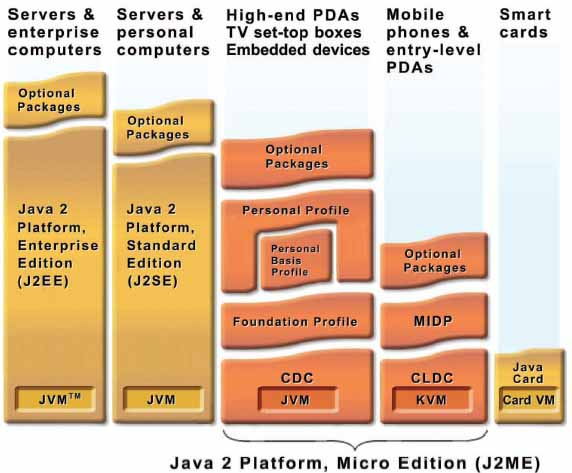
\includegraphics[width=\linewidth]{figures/j2meLayers}
    }
    \only<3>{
        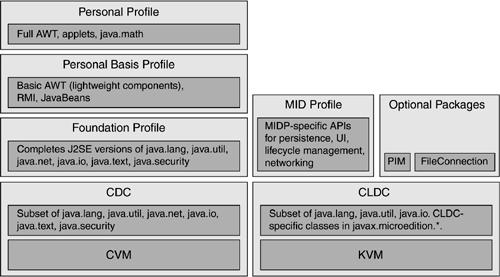
\includegraphics[width=\linewidth]{figures/j2meComponents}
    }
\end{frame}

\begin{frame}
    \frametitle{Programming in J2ME}

	\begin{itemize}
        \item Each mobile device has different hardware.
        \item Different KVM implementations (and bugs).
        \item ``Standard'' APIs implemented in different ways.
        \item A number of non-standard APIs and proprietary solutions.
        \item No system-level support for application testing.
	\end{itemize}

    \medskip
    \begin{center}\large\bfseries
    Conclusion:\\programming \emph{and testing} is difficult in J2ME.
    \end{center}
\end{frame}


\subsection[Scope]{Project scope} % ---------------------------------------------------------------- 

\begin{frame}
    \frametitle{Project scope}

	\begin{enumerate}
        \item Focus on capture-replay tests (GUI and other events).
        \item Should facilitate integration and regression tests in J2ME.
        \item Should work on emulators and actual devices.
	\end{enumerate}
\end{frame}

\begin{frame}[plain]
    \frametitle{Example of use}

    \hgraphics{figures/process1}
    \lbcaption{Capture-replay and regression testing.}
\end{frame}


\subsection[Related]{Related works} % --------------------------------------------------------------

\begin{frame}
    \frametitle{Related projects}

	\begin{itemize}
        \item J2ME Unit
        \item Sony-Ericsson Mobile JUnit
        \item Motorola Gatling
        \item CLDC Unit
        \item IBM Rational Test RT
        \item Research In Motion -- BlackBerry Fledge emulator
	\end{itemize}
\end{frame}



\section{RobotME} % --------------------------------------------------------------------------------

\begin{frame}
    And the ultimate answer is\ldots
    \vspace{2cm}
    \begin{center}\Huge\bfseries
    RobotME
    \end{center}
    \vspace{2cm}
    (of course the ultimate question still being ``what's $6\times 9$?'')
\end{frame}

\begin{frame}
    \frametitle{The core idea}

    \begin{itemize}
        \item Follow the regular capture-replay pattern.
        \item Cater for missing ``robot'' API by modifying the software at the \emph{bytecode} level.
        \item Verify replay-phase correctness by analysis of captured events.
    \end{itemize}
\end{frame}


\subsection[Injection]{Dynamic code injection} % ----------------------------------------------

\begin{frame}
    \frametitle{Dynamic code injection}

	\begin{itemize}
        \item Identify places which should generate an event (``injection~points'').
        \item Intercept parameters at injection points, injecting custom proxies.
	\end{itemize}
\end{frame}

\begin{frame}[fragile]
    \frametitle{Injection points: subclassing}

    Custom inheritance from system classes (subclassing).\\
    \texttt{Form}, \texttt{Canvas}, \texttt{MIDlet}\ldots{} 
    \begin{javablock}
public class MyMidlet extends MIDlet {
    protected void startApp() throws MIDletStateChangeException {
        // application code here.
    }
}
    \end{javablock}

    \bigskip
    We need to intercept the call to \texttt{startApp()} method.
\end{frame}

\begin{frame}[fragile]
    \begin{itemize}
        \item Make \texttt{MyMidlet} a subclass of \texttt{RobotMIDlet}?
        \begin{javablock}
public class MyMidlet extends RobotMIDlet {
        \end{javablock}
        {\tiny all methods virtual, multi-level inheritance}

        \pause
        \item Make a custom subclass \texttt{RobotMIDlet\$1} extend \texttt{MyMidlet}?
        \begin{javablock}
public class RobotMIDlet$1 extends MyMidlet {
        \end{javablock}
        {\tiny finalized classes, multi-level inheritance}

        \pause
        \item Use delegation pattern and alter the code of \texttt{startApp()}?
    \begin{javablock}
public class MyMidlet extends MIDlet {
    protected void startApp() throws MIDletStateChangeException {
        RobotME.event(this, STARTAPP_BEFORE);
        try {
            // application code here.
        } finally {
            RobotME.event(this, STARTAPP_AFTER);
        }
    }
}
    \end{javablock}
    {\tiny code bloat, goto, architectural flaws}
    \end{itemize}
\end{frame}

\begin{frame}[fragile]
    \frametitle{Injection points: references}

    Direct use of an object (reference tracking).\\
    \texttt{Command}, \texttt{Item} 
    \begin{javablock}
public class MyApplication {
    private static final Command MY_COMMAND =
        new Command("Cmd label", Command.OK, 1);

    public MyApplication() {
        Form f = new Form("Title");
        f.addCommand(MY_COMMAND);
    }
}
    \end{javablock}

    \bigskip
    We need to track the identity (and value) of commands.
\end{frame}

\begin{frame}[fragile]
    \begin{itemize}
        \item Substitute all constructors of \texttt{Form} with a 
        custom proxy?
        \begin{javablock}
Form f = new RobotME$Form("Title");
        \end{javablock}
        {\tiny clashes with custom inheritance}

        \pause
        \item Intercept all calls to \texttt{addCommand()}?
        \begin{javablock}
f.addCommand(RobotME.addCommand(f, MY_COMMAND));
        \end{javablock}
        {\tiny not too bad}
    \end{itemize}
\end{frame}

\begin{frame}[t,fragile]
    \frametitle{Injection points: listeners}

    Listeners (system callbacks).\\
    \texttt{ItemStateListener}, \texttt{CommandListener}, \texttt{ItemCommandListener} 
    \begin{javablock}
public class MyForm extends Form implements CommandListener {
    private final Command ADD_COMMAND;

    public MyClass {
        this.ADD_COMMAND = new Command("ADD", Command.OK, 1);
        this.setCommandListener(this);
    }

    public void commandAction(Command c, Displayable d) {
        // event handling code.
        if (c == ADD_COMMAND) {
            // ...do something.
        }
    }
...
    \end{javablock}

    \bigskip
    We need to track (and stimulate) commands for the listener. Note there
    is only \emph{one} listener on a \texttt{Form}.
\end{frame}

\begin{frame}[fragile]
    \begin{itemize}
        \item Intercept all calls to \texttt{setCommandListener()}?
        \begin{javablock}
this.setCommandListener(RobotME.setCommandListener(this, command));
        \end{javablock}
        {\tiny What if somebody uses ``=='' to compare listeners?}

        \pause
        \item How to remember the command received (if it's a dynamic reference)?\\
        {\tiny The reference changes between runs.}

        \pause
        \item How to generate an identical event dynamically?\\
        {\tiny The event should match the original \texttt{Display}/ \texttt{Form} pair.}
    \end{itemize}
\end{frame}

\begin{frame}[fragile]
    \frametitle{Examples of injected code}

    Original code (fragment):
    \begin{javablock}
final Form form = new Form("Questionnaire");
...
form.addCommand(CMD1_EXIT);
form.addCommand(CMD2_OK);
form.setCommandListener(this);

Display.getDisplay(this).setCurrent(form);
    \end{javablock}
\end{frame}

\begin{frame}[plain,fragile]
    Code modified for the recording phase:
    \begin{javablock}
Form form = new Form("Questionnaire");
...
form.addCommand(b); // NOTE: variable names have been obfuscated.
RobotMERecorder.getRecorderInstance().commandAddedToDisplayable(b, form);
form.addCommand(c);
RobotMERecorder.getRecorderInstance().commandAddedToDisplayable(c, form);
form.setCommandListener(this);
Display.getDisplay(this).setCurrent(form);
RobotMERecorder.getRecorderInstance().setCurrentDisplayable(form);
    \end{javablock}
    
    \medskip
    Code modified for the replay phase:
    \begin{javablock}
Form form = new Form("Questionnaire");
form.addCommand(b);
RobotMEReplaying.getReplayingInstance().commandAddedToDisplayable(b, form);
form.addCommand(c);
RobotMEReplaying.getReplayingInstance().commandAddedToDisplayable(c, form);
form.setCommandListener(this);
RobotMEReplaying.getReplayingInstance()
    .commandListenerSetOnDisplayable(this, form);
Display.getDisplay(this).setCurrent(form);
RobotMEReplaying.getReplayingInstance().setCurrentDisplayable(form);

RobotMEReplaying.getReplayingInstance().startReplaying();    
    \end{javablock}
\end{frame}

\begin{frame}[plain]
    \begin{center}
    A teraz przerwa dla miłośników granul.
    
    \bigskip\pause
\includegraphics[width=7cm]{figures/granules}
    \end{center}
\end{frame}

\subsection[Bytecode]{At the bytecode level}

\begin{frame}
    \begin{center}
    At the bytecode level\\
    {\color{blue} Java can be quite pleasant (and surprising!)}
    \end{center}
\end{frame}

\begin{frame}
    \frametitle{Java in assembler mode ;)}

    \begin{itemize}[<+->]
        \item The stack.
        \item Local variables.
        \item Opcodes and their mnemonics.
        \item Code verification.
    \end{itemize}
\end{frame}

\begin{frame}[fragile]
    \frametitle{Reverse-engineering Java code}

    \begin{javablock}
    public static final void method(int i)
    {
        System.out.println(i);
    }
    \end{javablock}

    \begin{center} $\downarrow$ \end{center}\pause

    \begin{codeblock}
    public static final void method(int i)
    {
        getstatic       #16  <Field PrintStream System.out>
        iload_0
        invokevirtual   #22  <Method void PrintStream.println(int)>
        return
    }
    \end{codeblock}
\end{frame}

\begin{frame}[fragile,plain]
    \frametitle{Reverse-engineering Java code}

    \begin{javablock}
    private final long sum(int a, int b) {
        return a + b;
    }

    public final void method() {
        System.out.println(sum(2, 50));
    }
    \end{javablock}

    \pause

    \begin{codeblock}
    private final long sum(int a, int b) {
        iload_1         
        iload_2         
        iadd            
        i2l             
        lreturn         
    }
    public final void method() {
        getstatic       #20  <Field PrintStream System.out>
        aload_0         
        iconst_2        
        bipush          50
        invokespecial   #26  <Method long sum(int, int)>
        invokevirtual   #28  <Method void PrintStream.println(long)>
        return          
    }    
    \end{codeblock}
\end{frame}

\begin{frame}[fragile,plain]
    \frametitle{Reverse-engineering Java code}
                                                   
    \begin{javablock}
    public final void method(int i) {
        switch (i) {
            case 1:
            case 25:
            case -5:
            case 1128:
                break;
            default:
                throw new RuntimeException();
        }
    }
    \end{javablock}

    \pause

    \begin{codeblock}
    public final void method(int i)
    {
        0    0:iload_1         
        1    1:lookupswitch default 47
              -5: 44
               1: 44
              25: 44
            1128: 44
        2   44:goto            55
        3   47:new             #16  <Class RuntimeException>
        4   50:dup             
        5   51:invokespecial   #18  <Method void RuntimeException()>
        6   54:athrow          
        7   55:return
    }    
    \end{codeblock}
    {\tiny Not the only possibility! }
\end{frame}

\begin{frame}[fragile,plain]
    \frametitle{Reverse-engineering Java code}

    \begin{javablock}
    public final int method(int i) {
        try {
            if (i == 0) {
                return 0;
            }
            if (i == 1) {
                return 1;
            }
            if (i == 2) {
                return 2;
            }
        } finally {
            System.out.println("aaa");
            System.out.println("bbb");
            System.out.println("ccc");
        }
        return -1;
    }
    \end{javablock}
    {\tiny What will this compile into? }
\end{frame}

\begin{frame}[fragile,plain]
    \tiny SUN's compiler
    \begin{javablock}
    public final int method(int i) {
        if (i == 0) {
            System.out.println("aaa"); System.out.println("bbb"); 
            System.out.println("ccc");
            return 0;
        }
        if (i == 1) {
            System.out.println("aaa"); System.out.println("bbb"); 
            System.out.println("ccc");
            return 1;
        }
        if (i == 2) {
            System.out.println("aaa"); System.out.println("bbb"); 
            System.out.println("ccc");
            return 2;
        } else {
            System.out.println("aaa"); System.out.println("bbb"); 
            System.out.println("ccc");
            return -1;
        }

exception_handler:
            System.out.println("aaa"); System.out.println("bbb"); 
            System.out.println("ccc");
        throw exception;
    }    
    \end{javablock}
\end{frame}

\begin{frame}[fragile,plain]
    \tiny IBM's compiler
    \begin{javablock}
    public final int method(int i) {
        int j;
        if (i != 0)
            goto  _L13;
        jsr local;
        j = 0;
        return j;
_L13:
        if (i != 1) goto _L27;
        jsr local;
        j = 1;
        return j;
_L27
        if (i != 2) goto _L2;
        jsr local;
        j = 2;
        return j;
_L2:
        jsr local;
        return -1;
local:
        System.out.println("aaa");
        System.out.println("bbb");
        System.out.println("ccc");
        ret;        
    }
    \end{javablock}
\end{frame}


\begin{frame}
    \hgraphics{figures/code-asm}
    \lbcaption{Bytecode-level changes.}
\end{frame}

\begin{frame}
    \hgraphics{figures/code}
    \lbcaption{\textsf{ASMLib} is used for preprocessing bytecode (statically).}
\end{frame}



\subsection[Maintenance]{Test maintenance}

\begin{frame}[containsverbatim]
    \frametitle{Test maintenance}

    Maintenance through \emph{human-comprehensible test scripts}.

    % TODO: check if this script is up-to-date.
    \bigskip
\begin{xmlblock}
<scenario>
  <event timestamp="1000">
      <displayable-changed title="Hello screen" type="TEXTBOX" />
  </event>
    
  <event timestamp="2000">
      <command cmdLabel="Start app" displayableTitle="Hello screen" />
  </event>
    
  <event timestamp="3000">        
      <textbox-modification assertion="true" strongAssertion="true" 
                            string="I like testing" />
  </event>
</scenario>
\end{xmlblock}

\end{frame}


\subsection[Prototype]{Proof-of-concept prototype} % -----------------------------------------------

\begin{frame}[plain]
	\frametitle{Time for a live demo!}

    \lbcaption{Server console.}
    \rbcaption{Emulator window.}

    \fxygraphics{12.4}{0.5}{right}{bottom}{width=5cm}{figures/1}
    \fxygraphics{0.2}{8.4}{left}{top}{width=12.4cm}{figures/2}
\end{frame}

\section*{Summary} % -------------------------------------------------------------------------------

\begin{frame}[plain]
    \frametitle{Summary}

    \begin{itemize}
        \item Testing is difficult in J2ME.
        \item Bytecode manipulation can provide a substitute 
        for the required API functions. 
    \end{itemize}

    \medskip
    \begin{itemize}
        \item The prototype a bit gritty, but functional.
    \end{itemize}
\end{frame}

\begin{frame}[plain]
    \frametitle{Little victories}

    \begin{itemize}
        \item Springer LNCS publication (10th BIS conference).
        \item UAM Foundation --- ``Pomysł na biznes'' competition.
    \end{itemize}
\end{frame}

\begin{frame}[plain]
	\begin{center}
	Thank you for your attention.
	\end{center}
\end{frame}

\end{document}
